% !TeX root = main.tex
\documentclass[a4paper,12pt,twocolumn]{article}

% Packages
\usepackage[utf8]{inputenc}
\usepackage[T1]{fontenc}
\usepackage[backend=biber,style=abnt]{biblatex}
\usepackage{amsmath, amssymb}
\usepackage{graphicx}
\usepackage{hyperref}
\usepackage{geometry}
\geometry{margin=1in}
\usepackage{listings}
\usepackage{minted}
\usepackage{color}

% Title Page
\title{Algorithm Implementation Report}
\author{Rafael Ramildes Ferreira \\ \href{mailto:rafaelramildes@hotmail.com}{\texttt{rafaelramildes@hotmail.com}}}
\date{Florianópolis, SC \\ 2025}

\bibliography{bibliography}

% Define a custom color
\definecolor{backcolour}{rgb}{0.95,0.95,0.92}
\definecolor{codegreen}{rgb}{0,0.6,0}
\definecolor{codeblue}{rgb}{0.2,0.4,0.8}
\definecolor{codeyellow}{rgb}{0.8, 0.6, 0.0}
\definecolor{darkgreen}{rgb}{0.0, 0.4, 0.0}
\definecolor{codeorange}{rgb}{1.0, 0.6, 0.0}
\definecolor{codered}{rgb}{0.8, 0.0, 0.0}
\definecolor{codepurple}{rgb}{0.6, 0.0, 0.6}
\definecolor{lightblue}{rgb}{0.6, 0.8, 1.0}

\lstdefinestyle{myStyle}{
    backgroundcolor=\color{backcolour},   
    commentstyle=\color{codegreen},
	keywordstyle=[1]\color{blue},
	keywordstyle=[2]\color{codeyellow}\bfseries,
	keywordstyle=[3]\color{codepurple},
	keywordstyle=[4]\color{codeblue},
	keywordstyle=[5]\color{codered}\bfseries,
	stringstyle=\color{codepurple},
    basicstyle=\ttfamily\tiny,
    breakatwhitespace=false,         
    breaklines=true,                 
    keepspaces=true,                                   
    showspaces=false,                
    showstringspaces=false,
    showtabs=false,                  
    tabsize=2,
}

% Use \lstset to make myStyle the global default
\lstset{style=myStyle}

\begin{document}

\maketitle
% \noindent\rule{\textwidth}{0.5pt}
% \tableofcontents
% \newpage

\section*{Introduction}

Throughout the semester, some of the studied algorithms and data structures were implemented as a course assignment. They were initially implemented in C. The Gale-Shapley Algorithm was implemented in Python, for the built-in hash map (\texttt{dict}). Later C++ was used to implement the binary heap and binary tree, to make use of the class definition as a template.

The whole implementation as well as the \LaTeX\ source code and the report as a pdf are available on GitHub at \url{https://github.com/Rafael-Ramildes-Ferreira/Algorithms}

The Implementation of the first two algorithms are explained and compared in \autoref{sec:sorting}. The Gale-Shapley algorithm is explained in \autoref{sec:gale-shapley}. The binary heap implementation and heap sort are discussed in \autoref{sec:binary-heap}. Finally, the binary tree implementation is presented in \autoref{sec:binary-tree}.

\section{Basic Sorting Algorithms}
\label{sec:sorting}

The basic sorting algorithms implemented in this assignment are Insertion Sort and Merge Sort. The implementation of these algorithms is done in C and a makefile is provided to compile each of the algorithm's code.
The code divides the author's implementation and the implementation proposed by \cite{cormenIntroductionAlgorithms2022} by adding the sufix \verb|_book| in the function name.
The author's implementation was made by memory from the algorithm presented in class.
In addition, for comparing the two implementations, Google's Benchmark library is used.

The file \verb|Benchmarking.md| contains the results of the benchmarking tests.
Additionally, there is a python script that plots the execution time of the algorithms.

In \autoref{sec:insertion-sort} and \autoref{sec:merge-sort} is an explaination of this work's proposed implementation of the insertion and merge sort, respectively, and how they differ from the book's implementation. \autoref{sec:benchmark} presents the results of the benchmarking tests and compares the two implementations.

\subsection{Insertion Sort}
\label{sec:insertion-sort}
The insertion sort algorithm uses a insertion of a new element in a sorted list. This element is inserted before the smallest element that is greater than it, keeping the list sorted. It is used to sort any list \verb|A[1..n]| doing a insertion of the \verb|i|th element in the sublist \verb|A[1..i-1]|. Starting with \verb|i| equal 2, and increasing \verb|i| at every insertion, until \verb|i| is equal to \verb|n|, the end result is the sorted version of the list \verb|A[1..n]|.

Firstly, the algorithm was implemented using recursion. From a full size list \verb|A[1..n]|, the algorithm calls itself with a smaller list \verb|A[1..n-1]|. The base case is when the list has two elements, where the function decides the order of the elements. When it happens, the algorithm starts working down the program stack, inserting the last element in the sorted list. The insertion function loops through the list to find the correct position for the new element. The algorithm is implemented in \verb|insertion.c|.

\textcite{cormenIntroductionAlgorithms2022} defines the insertion sort algorithm with two nested loops: the outer loop for each value of \verb|i|; the inner loop is analogous with the insertion function of the previous implementation. This method avoids build up the program memory stack and avoid the overhead of function calls. Inspite of this, both implementation present a very similar excecution time and number of operations.

\subsection{Merge Sort}
\label{sec:merge-sort}
The merge sort is performed by merging two sorted lists.
To make these two sorted lists, the merge sort is recursively called on a sublist made by half the original list (\verb|A[1..n/2]| and \verb|A[n/2+1..n]|).
The base case is when the sublist has one or two element, where is either already sorted, in the case of one element, or the function decides which element cames first, based on a simple if statement.
The merge sort algorithm is implemented in \verb|merge.c|.

The merging part is implemented in function \verb|merge|, just walking through each sublist and copying the smaller element into a new list.
When one of the sublists is empty, the remaining elements of the other sublist are copied to the new list.
The recursively merge sort function is called \verb|merge_sort|, which calls itself with the two sublists until the base case is reached.
It needs to copy both halves, allocating memory for each sublistm and make sure they're sorted byt calling the \verb|merge_sort| function on each half.
Then it merges the two sorted halves into a new list, which is returned to the previous call.

The implementation proposed in the book is very similar:
also uses two functions, one for the merge and another for the merge sort.
The main diference is that the book performes the allocation and copying of the list in the merge function, which is not recursive, an thus has less memory overhead.
The merge sort function, then has pointers to the beginning and end of the list to know the portion where the list needs to be sorted.
In the book implementation, there is only one base case, when the list has one element, which is already sorted.

It performed worse on time, and had more malloc calls.
The reduction on the number of base cases may be the cause of the increase in malloc calls, since for both, one call is made for every sublist of size greater than two, but only the book implementation calls for sublists of size two. However, the time taken by the malloc calls alone, is not enough to justify the increase in time, as it can be seen in the results of the benchmark.

\subsection{Analysis}
\label{sec:benchmark}
These algorithms run time were measured using Google's Benchmark library.
The benchmarks can be executed by running the \verb|make <source_name> OPTIONS=| \verb|BENCHMARKING| command in the terminal,
as shown in the ReadME file.
Some of the results are shown in the \verb|Benchmarking.md| file.
Also, a python script is provided to plot the results of the benchmark.

The benchmarks use pregenerated random lists of 1000 elements.
This same list is subdivided in smaller lists during the tests.
The results will depend on the machine running the algorithms, but the relative performance of the algorithms should be similar.

Even though the merge sort has a better theoretical time complexity, the insertion sort performed better in practice.
This could be due to caching effects, helping the insertion sort to perform better on smaller lists,
due to the overhead of the memory allocation in the merge sort,
or simply the lists are not large enough for the higher complexity term to dominate the runtime.

The lists used in the benchmark not being generated at runtime may cause them to be repetitive, and thus, take advantage of the cache.
The merge sort is always allocating new memory and copying the elements to the new list, so caching may not be used as effectively as in the insertion sort.

The idea that the \verb|malloc| overhead could be delaying the merge sorted was tested and shows this is at least not the whole cause.
In the \verb|merge.c| file, the \verb|malloc| was rewritten to allow for the benchmark library to record the amount of time and  memory allocated.
The \verb|malloc.c| file runs a benchmark of the \verb|malloc| calls.
It repeats the same number of calls with the average size allocated in the merge sort.
The result of this benchmark is also in the \verb|Benchmark.md| file

\begin{figure}[htbp]
	\centering
	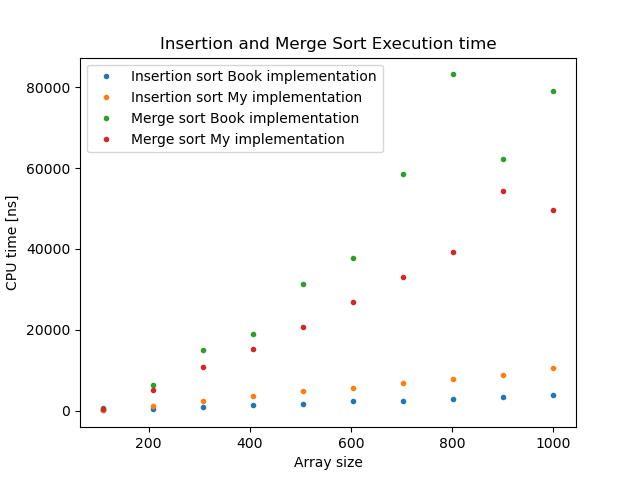
\includegraphics[width=\linewidth]{Fig/Insertion_Merge_comp.png}
	\caption{Execution time of the Insertion and Merge sort compared between this work's implementation and the book's implementation.}
\end{figure}

% \begin{figure}[htbp]
% 	\centering
% 	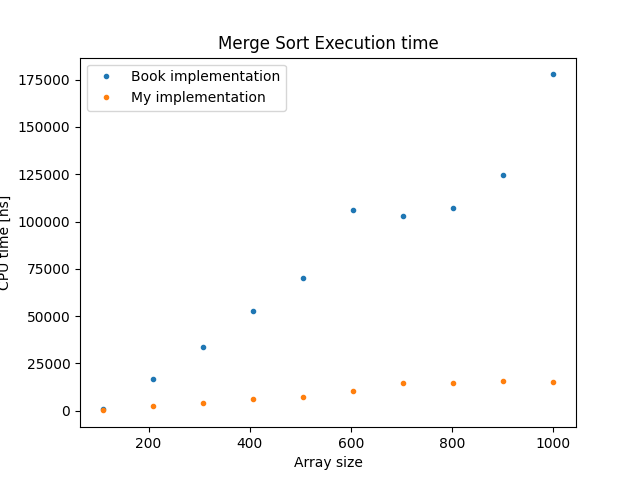
\includegraphics[width=\linewidth]{Fig/Merge_comp.png}
% 	\caption{Execution time of the Merge sort compared between this work's implementation and the book's implementation.}
% \end{figure}


\section{Gale-Shapley Algorithm}
\label{sec:gale-shapley}

The Gale-Shapley algorithm, was implemented in Python, to use the built-in hash map (\texttt{dict}).
It is used to make accesses in constant time.
The Man needs to find a Woman based on the rank, while the Woman need to find a Man's rank when receiving proposals. 
So each have a different implementation as is shown below.
The Man also need to record the next rank he need to search next, 
in case the Woman he is married to marries to another Man.

\begin{lstlisting}[float=htbp,language=Python]
class Men(Person):
	def __init__(self) -> None:
		self.married: Women = None
		self.preference_list: dict[int,Women] = None 
		# Indexed by rank, to quickly find the next ranked woman
		self.search_index: int = 0

	def begin(self, pair: list[Women]) -> None:
		self.preference_list = {}
		preference: list[int] = list(range(len(pair)))
		shuffle(preference)
		for i,target in enumerate(pair):
			self.preference_list[preference[i]] = target
			
class Women(Person):
	def __init__(self) -> None:
		self.married: Men = None
		self.rank: dict[Men,int] = None	
		# Indexed by man, to quickly find if he has higher rank than the currently married

	def begin(self, pair: list[Men]) -> None:
		self.rank = {}
		preference: list[int] = list(range(len(pair)))
		shuffle(preference)
		for i,target in enumerate(pair):
			self.rank[target] = preference[i]
\end{lstlisting}

The class Person just have code that is repeated in both Man and Woman.
Mostly dunder functions to allow for hashing the object so it can be used as a key in a dictionary.

\begin{lstlisting}[float=htbp,language=Python]
class Person(ABC): 
	def __init__(self) -> None:
		self.married: Person = None

	def __hash__(self) -> int:
		return id(self)

	def __eq__(self, other) -> bool:
		return self is other
\end{lstlisting}

A class was implemented to handle the society, called Church, which contains an equal number of men and women.
It creates each Man and Woman and initializes each of them.
Initializing a Man or Woman consists of creating a preference list, which is a random list of the other sex.
This initialization is shown above in the methods \verb|begin|, the Church implementation is shown next page.

\begin{lstlisting}[float=htbp,language=Python]
class Church:
	"""This class encapsulates a society with a equal number of men and women"""
	def __init__(self, n : int = 5):
		self.men: list[Men] = [Men() for _ in range(n)]
		self.women: list[Women] = [Women() for _ in range(n)]
		self.marriage_list: list[tuple[Men,Women]] = []

		for man in self.men:
			man.begin(self.women)

		for woman in self.women:
			woman.begin(self.men)
\end{lstlisting}

The Gale-Shapley algorithm is implemented as a method of the Church class.
While there are free Mans, it takes the first free Man and searches for Women,
going down the ranks until he finds a Woman that is not married or that is married to a Man of lower rank.
If the Woman is married to a lower ranked Man, she will switch to the new Man and her ex-husband will become free.
The rank is implemented so the smallest numbers are higher ranks.

\begin{lstlisting}[float=htbp,language=Python]
class Church:
 	...
	def gs_algorithm(self,men:list[Men],women:list[Women]) -> None:
		free_men: list[Men] = men.copy()
		while len(free_men) > 0:
			man: Men = free_men[0]
			while man.search_index < len(women):
				woman = man.preference_list[man.search_index]
				man.search_index += 1

				# She has no choice
				if woman.married == None:
					self.marry(man,woman)
					free_men.pop(0)
					break
				
				# Small rank is better
				elif woman.rank[woman.married] > woman.rank[man]:
					free_men.append(woman.married)
					self.marry(man,woman)
					free_men.pop(0)
					break
\end{lstlisting}

The marry method just sets the married attribute of both Man and Woman and appends the couple to the marriage list.
The code below shows the implementation.

\begin{lstlisting}[float=htbp,language=Python]
class Church:
 	...
	def marry(self, man: Men, woman: Women) -> None:
		man.married = woman
		woman.married = man

		self.marriage_list.append( (man,woman) )
\end{lstlisting}

There is also a method to validate the marriages, checking if no one is married to more than one Person,
and if everyone is married.
For every Man, it checks if all higher ranked Women are married to higher ranked Man.
It would not be a stable matching if a higher ranked Woman is married to a lower ranked Man.

\begin{lstlisting}[float=htbp,language=Python]
class Church:
 	...
	def validate_marriages(self) -> None:
		"""Check if every member of a given gender is married
		and if two or more are not married to the same person"""

		assert(len(self.men) == len(self.women))

		for man in self.men:
			assert(man.married != None)			
			# Every man should be married
			assert(man == man.married.married)	
			# The spouse of the man's spouse should be himself
			i: int = man.search_index - 1
			while i >= 0:
				# Asserts that every higher rank woman is married to a higher rank man
				woman: Women = man.preference_list[i]
				assert(woman.rank[woman.married] <= woman.rank[man]) 
				# Higher rank is smaller number
				i -= 1
\end{lstlisting}

\section{Binary Heap}
\label{sec:binary-heap}
\subsection{Binary Heap Implementation}
Analyze the results, discuss their significance, and mention any challenges faced.

\subsection{Heap Sort}
Summarize the key findings and suggest possible future work.


\section{Binary Tree}
\label{sec:binary-tree}

% \section*{References}
\printbibliography

\end{document}